\subsection{Glyph: \glyph{Not}}
\label{sec:af:not}

The glyph \glyph{not} is used to denote that the \glyph{AN} linked as input cannot influence the target activity.

\begin{glyphDescription}
 \glyphSboTerm SBO:0000238 ! not.
 \glyphIncoming One \glyph{logic arc} (\sect{af:logicArc}).
 \glyphOutgoing  One \glyph{logic arc} (\sect{af:logicArc}) or one of the modulation arcs (\sect{af:arcs}).
 \glyphContainer A \glyph{not} operator is represented by a circular shape containing the word ``NOT''.
The shape is linked to two ports, that are small arcs attached to the centres of opposite sides of the shape, as shown in \fig{af:not}.
The incoming \glyph{logic arc} (\sect{af:logicArc}) is linked to the extremity of the leftmost or uppermost port, while the outgoing \glyph{logic arc} (\sect{af:logicArc}) or modulation arc (\sect{af:arcs}) is linked to the extremity of the rightmost or bottommost port.
 \glyphLabel None.
 \glyphAux None.
 \end{glyphDescription}

\begin{figure}[H]
  \centering
  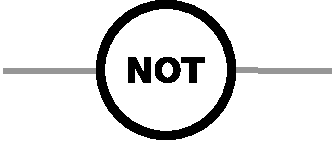
\includegraphics[scale = 1]{images/build/not.pdf}
  \caption{The \AF glyph for \glyph{not}.}
  \label{fig:af:not}
\end{figure}
